\documentclass[11pt,a4paper]{article}
\usepackage[margin=2.4cm]{geometry}
\usepackage{booktabs,graphicx,xcolor,amsmath,array,caption,longtable}
\usepackage[colorlinks=true,linkcolor=Blue,urlcolor=Blue]{hyperref}
\definecolor{Blue}{HTML}{1D4ED8}
\definecolor{Good}{HTML}{15803D}
\definecolor{Bad}{HTML}{B91C1C}
\definecolor{Grey}{HTML}{5B6474}
\newcommand{\gd}[1]{\textcolor{Good}{#1}}
\newcommand{\bd}[1]{\textcolor{Bad}{#1}}
\newcommand{\ci}[1]{{\footnotesize\textcolor{Grey}{#1}}}
\captionsetup{font=small,labelfont=bf}
\setlength{\parskip}{5pt}\setlength{\parindent}{0pt}
\renewcommand{\arraystretch}{1.15}

\title{\vspace{-1.6cm}\textbf{Guidance for CoBit bitstream diffusion}\\[2pt]
\large What we ran, what we found, and what changed}
\author{\normalsize Rares Grozavescu}
\date{\normalsize 3 September 2026 \quad$\cdot$\quad TinyGSM $\rightarrow$ GSM8K \quad$\cdot$\quad 329 runs, 107 A100-hours}
\begin{document}\maketitle\vspace{-0.6cm}

\hrule\vspace{6pt}
\textbf{Summary in five lines.}
\begin{enumerate}\itemsep1pt
\item Under deterministic sampling, all three guidance methods help: CFG $+0.081$, AutoGuidance $+0.066$, Self-Guidance $+0.048$.
\item Self-Guidance is \emph{not} a numerical-solver artefact --- a correctly implemented second-order solver (Heun) gives nothing at matched cost.
\item Switching on stochastic churn --- a sampler flag costing \emph{no extra forward passes} --- raises the plain baseline by $+0.120$, more than any guidance method delivers.
\item Under churn, CFG survives but must be re-tuned ($w{=}12\rightarrow2$); AutoGuidance reverses; Self-Guidance reverses at every scale tested.
\item Guidance and majority voting compose \emph{additively}, but at equal forward passes extra samples remain the better buy.
\end{enumerate}
\vspace{2pt}\hrule

\section{Setup}
CoBit is a continuous diffusion language model over \emph{bitstreams}: it denoises a real-valued vector whose coordinates are bit probabilities, and decodes to tokens at the end. We evaluate on GSM8K (grade-school maths word problems), zero-shot from a TinyGSM-trained checkpoint. The model writes a short Python program; we execute it in a sandbox and compare the returned number to the gold answer. The metric throughout is \textbf{exact match}.

Three guidance mechanisms are compared. Writing $D$ for the model's predicted clean bit-probabilities:
\[
\underbrace{D_u + w(D_c-D_u)}_{\textbf{CFG}}\qquad
\underbrace{D_{\text{bad}} + w(D_{\text{good}}-D_{\text{bad}})}_{\textbf{AutoGuidance}}\qquad
\underbrace{D + w\,(D_t - D_{\text{prev}})\cdot\tfrac{\delta}{\Delta\log\sigma}}_{\textbf{Self-Guidance}}
\]
CFG contrasts a conditional against an unconditional (null-prompt) branch; AutoGuidance contrasts the final checkpoint against a deliberately weaker earlier one; Self-Guidance contrasts predictions at adjacent noise levels. CFG and AutoGuidance each need \emph{two} network evaluations per step; Self-Guidance reuses a cached prediction and is free.

\textbf{Statistics.} Screening runs use a fixed 250-problem prefix and one seed. Every number quoted below is \textbf{confirmation grade}: all 1319 GSM8K test problems, three seeds, with per-problem paired bootstrap intervals (20{,}000 resamples). Pairing removes problem-difficulty variance, which is what makes 2-point effects resolvable at this sample size.

\textbf{The parameter $\gamma$} controls EDM-style \emph{stochastic churn}: at each step the state is partially re-noised before being denoised again, with $s_{\text{churn}}=\gamma\,(\text{NFE}-1)$, capped at $\sqrt2-1$. Crucially this adds \emph{no} network evaluations --- measured at 256 NFE, ${\sim}94$\,s and 2.31\,GB for every $\gamma$ we tested.

\section{What we ran}
\begin{center}\footnotesize
\begin{tabular}{llrl}
\toprule
\textbf{Stage} & \textbf{Experiment} & \textbf{Cells} & \textbf{Question} \\
\midrule
\textit{Guidance at} $\gamma=0$
 & \texttt{cfg\_coarse}, \texttt{cfg\_high} & 18 & CFG scale, 0.25--30 \\
 & \texttt{ag}, \texttt{ag\_high}, \texttt{ag\_ema} & 50 & AutoGuidance badness $\times$ scale \\
 & \texttt{sg}, \texttt{sg\_delta}, \texttt{sg\_mf} & 52 & Self-Guidance variant, $\delta$, matched filter \\
 & \texttt{cfg/ag/sg\_confirm} & 36 & full-size confirmation, 3 seeds \\
 & \texttt{factorial\_confirm} & 36 & all 12 method combinations \\
 & \texttt{nfe} & 28 & quality vs compute, 8--512 steps \\
 & \texttt{null\_ablation} & 3 & sensitivity to the CFG null \\
\midrule
\textit{Controls}
 & \texttt{solver\_control} & 15 & is Self-Guidance just 2nd-order integration? \\
 & \texttt{compute\_control} & 4 & disjoint seeds for majority voting \\
 & \texttt{repro} & 4 & did the evaluation change move any number? \\
\midrule
\textit{Stochasticity}
 & \texttt{stoch\_screen} & 20 & $\gamma$ screen, 4 methods \\
 & \texttt{stoch\_confirm} & 36 & full-size confirmation \\
 & \texttt{churn\_anatomy} & 21 & re-tune CFG at $\gamma{=}0.3$; can SG be rescued? \\
\midrule
 & \textbf{total} & \textbf{329} & \\
\bottomrule
\end{tabular}
\end{center}

Two analyses cost \emph{no} GPU time because the per-problem executed answers were already recorded: the compute-matched majority-vote controls (\S5) and the guidance$\times$voting composition test (\S6).

\section{Guidance under deterministic sampling}
Each method at its own tuned operating point, against a single baseline sample.

\begin{center}\small
\begin{tabular}{lrrlr}
\toprule
\textbf{Configuration} & \textbf{Exact match} & \textbf{$\Delta$} & \textbf{95\% CI} & \textbf{NFE} \\
\midrule
CFG $w{=}12$              & 0.2196 & \gd{$+0.0811$} & \ci{[$+0.0675,+0.0953$]} & 1024 \\
AutoGuidance $w{=}15$     & 0.2047 & \gd{$+0.0662$} & \ci{[$+0.0533,+0.0794$]} & 1024 \\
SG-prev $w{=}2$           & 0.1868 & \gd{$+0.0483$} & \ci{[$+0.0392,+0.0576$]} & \textbf{512} \\
SG-exact $w{=}1$          & 0.1233 & \bd{$-0.0152$} & \ci{[$-0.0220,-0.0083$]} & 1024 \\
\midrule
baseline                  & 0.1385 & --- & --- & 512 \\
\bottomrule
\end{tabular}
\end{center}

Two details matter more than the ranking. \textbf{SG-prev runs at the baseline's cost} --- it is the only free method. And \textbf{SG-exact, which costs twice as much, is worse than doing nothing}: the cheap approximation is not approximating the expensive one.

\paragraph{Combinations destroy the model.} The full $2\times2\times3$ factorial (Fig.~\ref{fig:fact}) shows every combination is worse than its best component, and CFG${+}$AutoGuidance collapses to \textbf{0.0005} --- essentially no correct answers. The interaction is $-0.166$. Diagnostically the guidance-to-score ratio rises from 0.20 (CFG alone) to 0.86 (CFG${+}$AG) to 11.6 (three-way): stacking multiplies the amplification and drives every bit to a hard 0 or 1.

\begin{figure}[htbp]\centering
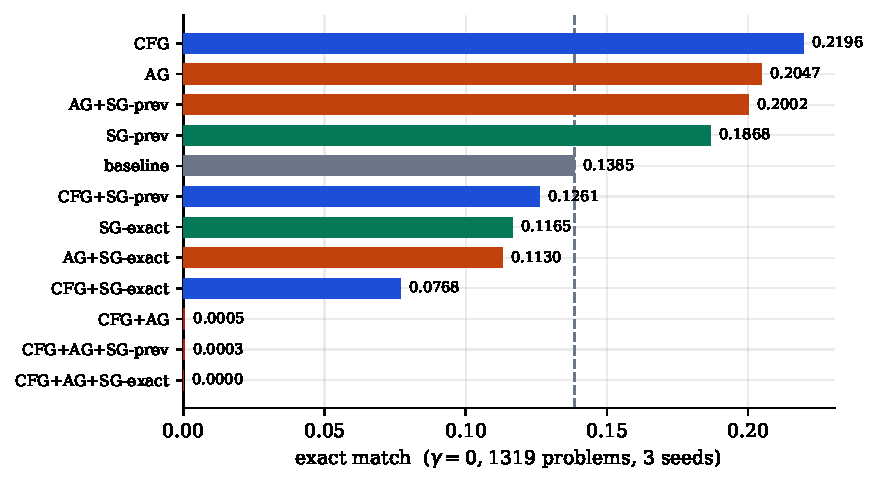
\includegraphics[width=.66\textwidth]{fig/fig5_factorial.pdf}
\caption{All twelve factorial conditions, $\gamma=0$. Red bars are the collapsed combinations. Dashed line is the unguided baseline.}\label{fig:fact}
\end{figure}

\section{Is Self-Guidance really guidance?}
SG-prev's direction is a difference between consecutive predictions, divided by the log-$\sigma$ spacing --- an amplified finite-difference derivative. That is structurally what a second-order ODE solver computes, from the same two quantities, so ``guidance'' and ``better numerical integration'' predicted the same $+0.048$.

We implemented Heun (a genuine second-order solver) and compared at \emph{measured} forward passes. This mattered: the recorded NFE field counted only guidance branches and was blind to solver order, under-reporting Heun by $2\times$. Instrumenting \texttt{model.forward} gave DDIM exactly 1.00 evaluations/step and Heun $2N{-}1$.

\begin{figure}[htbp]\centering
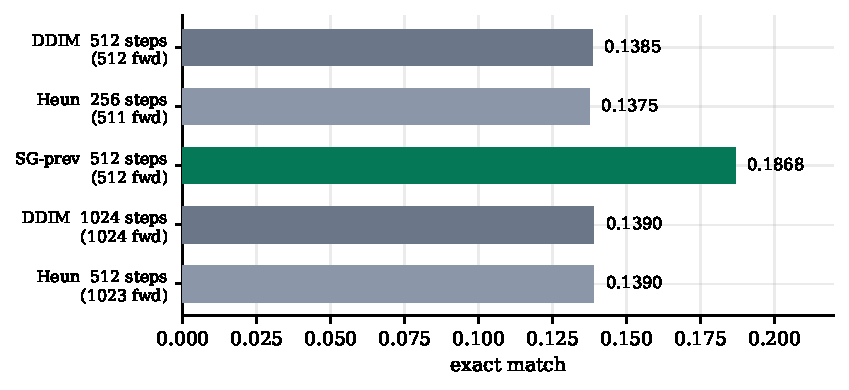
\includegraphics[width=.72\textwidth]{fig/fig3_solver.pdf}
\caption{Solver control at matched forward passes. Heun matches DDIM at both budgets; SG-prev does not.}\label{fig:solver}
\end{figure}

SG-prev beats Heun by \gd{$+0.0493$} \ci{[$+0.0402,+0.0586$]} at identical cost, while Heun differs from DDIM by $-0.0010$ \ci{[$-0.0030,+0.0010$]} (not significant). Doubling DDIM's steps also does nothing ($0.1390$ vs $0.1385$). \textbf{The solver hypothesis is rejected.} What SG-prev encodes is still unknown.

\section{Stochastic churn changes everything}
Every result above was measured with churn disabled. It should not have been held fixed.

\begin{figure}[htbp]\centering
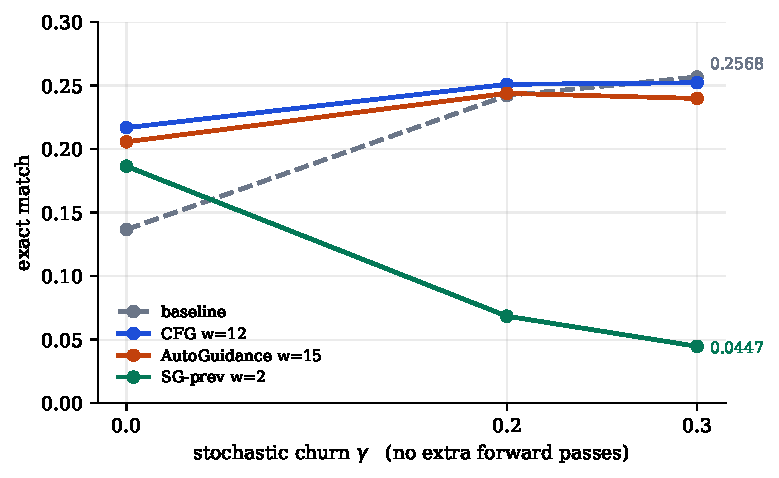
\includegraphics[width=.72\textwidth]{fig/fig1_gamma.pdf}
\caption{Exact match against churn $\gamma$. The unguided baseline (dashed) climbs past every guided line. SG-prev inverts completely. 1319 problems, 3 seeds.}\label{fig:gamma}
\end{figure}

The unguided baseline gains \gd{$+0.1200$} \ci{[$+0.1056,+0.1350$]} going from $\gamma{=}0$ to $\gamma{=}0.3$ --- larger than any guidance effect in this study, at no additional cost. Measured against the \emph{same-$\gamma$} baseline, the guidance methods behave very differently:

\begin{center}\small
\begin{tabular}{lccc}
\toprule
\textbf{vs.\ same-$\gamma$ baseline} & $\gamma=0$ & $\gamma=0.2$ & $\gamma=0.3$ \\
\midrule
CFG $w{=}12$          & \gd{$+0.0801$} & $+0.0088$ \ci{n.s.} & $-0.0045$ \ci{n.s.} \\
AutoGuidance $w{=}15$ & \gd{$+0.0690$} & $+0.0018$ \ci{n.s.} & \bd{$-0.0169$} \\
SG-prev $w{=}2$       & \gd{$+0.0498$} & \bd{$-0.1736$}      & \bd{$-0.2120$} \\
\bottomrule
\end{tabular}
\end{center}

\paragraph{But CFG was mis-tuned, not superseded.} $w{=}12$ was chosen at $\gamma{=}0$. Sweeping the scale \emph{at} $\gamma{=}0.3$ separates ``guidance stops working'' from ``guidance is tuned for the wrong regime''. It is the second: $w{=}2$ gives $0.2757$, \gd{$+0.0190$} \ci{[$+0.0068,+0.0316$]} over the plain stochastic baseline.

\begin{figure}[htbp]\centering
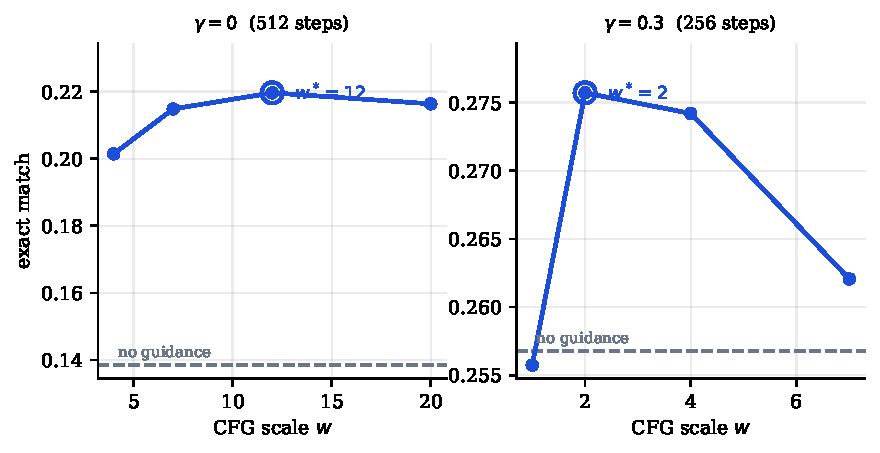
\includegraphics[width=.92\textwidth]{fig/fig2_cfgscale.pdf}
\caption{The optimal CFG scale moves from $w^*\!\approx\!12$ to $w^*\!\approx\!2$ when churn is switched on, and the gain shrinks from $+0.080$ to $+0.019$. \textbf{A guidance scale quoted without its sampler regime is under-specified.}}\label{fig:cfgscale}
\end{figure}

\paragraph{Self-Guidance cannot be rescued.} If the direction were right and only the magnitude wrong, shrinking the scale should restore it. It does not: at $\gamma{=}0.3$, $w=0.06/0.125/0.25$ give $-0.0131/-0.0286/-0.0551$ --- still harmful $33\times$ below the $\gamma{=}0$ optimum, and harm \emph{linear in $w$}, the signature of a systematically wrong direction rather than amplified noise. Two mechanisms are already excluded by the traces: the spacing normaliser is unchanged across $\gamma$, and $\log\sigma$ remains monotone. Working hypothesis (untested): churn re-noises the state each step, so the cached prediction comes from a strictly noisier point and the difference acquires a consistent backward component.

\section{Compute: is guidance worth its extra evaluations?}
CFG and AutoGuidance double the network evaluations per sample. The honest comparison spends those same evaluations on \emph{more samples} and combines them by majority vote --- deployable, unlike the pass@$k$ oracle bound.

\begin{center}\small
\begin{tabular}{lrrr}
\toprule
\textbf{Arm} ($\gamma=0.3$) & \textbf{NFE} & \textbf{Samples} & \textbf{Exact match} \\
\midrule
baseline, single sample & 256 & 1 & 0.2568 \\
baseline maj@2          & 512 & 2 & 0.2881 \\
baseline maj@3          & 768 & 3 & \textbf{0.3146} \\
CFG $w{=}2$, single     & 512 & 1 & 0.2757 \\
CFG $w{=}2$ maj@2       & 1024 & 2 & 0.3060 \\
\bottomrule
\end{tabular}
\end{center}

\begin{figure}[htbp]\centering
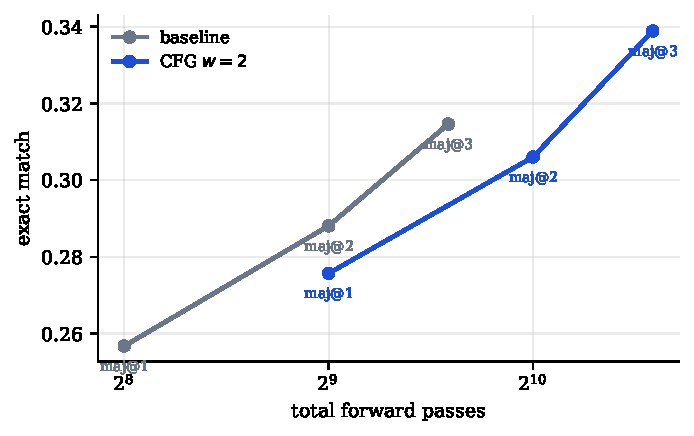
\includegraphics[width=.62\textwidth]{fig/fig4_voting.pdf}
\caption{Guidance and voting compose additively: voting adds $+0.0313$ to the baseline and $+0.0303$ to CFG --- statistically the same increment, so the two mechanisms are independent.}\label{fig:vote}
\end{figure}

\textbf{The verdict depends on what is held fixed}, and these must not be collapsed into one ``compute'' number:
\begin{center}\small
\begin{tabular}{@{}p{3.4cm}p{5.3cm}rl@{}}
\toprule
\textbf{Held fixed} & \textbf{Comparison} & \textbf{$\Delta$} & \textbf{Verdict} \\
\midrule
number of samples \newline \ci{(latency-bound)} & CFG maj@2 $-$ baseline maj@2 & \gd{$+0.0179$} & \gd{guidance wins} \\
 & \ci{[$+0.0023,+0.0339$]} & & \\[2pt]
forward passes & CFG maj@2 (1024) $-$ baseline maj@3 (768) & $-0.0086$ & inconclusive$^\ast$ \\
 & \ci{[$-0.0258,+0.0088$]} & & \\
\bottomrule
\end{tabular}
\end{center}
{\footnotesize $^\ast$and the baseline used 25\,\% \emph{less} compute to achieve it.}

For a latency-bound single-stream deployment, guidance is worth it. For a throughput-bound one, extra samples are the better buy. Fig.~\ref{fig:nfe} shows the same story at $\gamma=0$ across the NFE range.

\begin{figure}[htbp]\centering
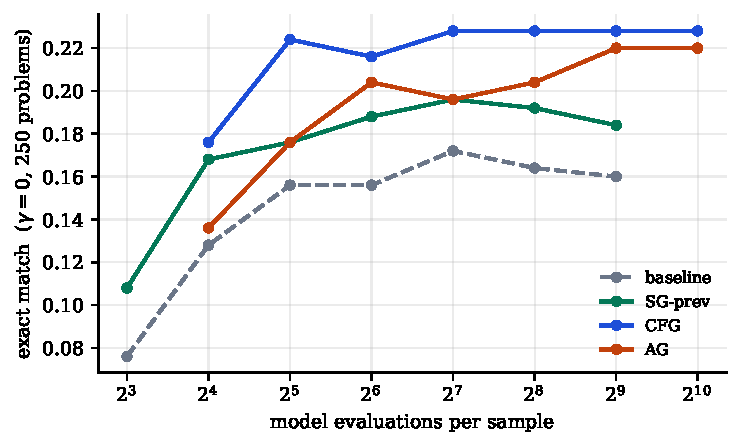
\includegraphics[width=.62\textwidth]{fig/fig6_nfe.pdf}
\caption{Quality against model evaluations at $\gamma=0$ (250-problem screen). The baseline plateaus near 0.17; guidance buys a higher plateau, not a faster one.}\label{fig:nfe}
\end{figure}

\section{What is established, and what is not}
\begin{center}\small
\begin{tabular}{llll}
\toprule
\textbf{Claim} & \textbf{$\gamma=0$} & \textbf{$\gamma=0.3$} & \textbf{Status} \\
\midrule
CFG helps                          & $+0.0811$ & $+0.0190$ ($w{=}2$) & \gd{survives, re-tuned} \\
AutoGuidance helps                 & $+0.0690$ & $-0.0169$ & \bd{reverses} \\
SG-prev helps                      & $+0.0498$ & $-0.2120$ & \bd{reverses at every scale} \\
SG-prev is a solver effect         & --- & --- & \bd{rejected} \\
Guidance beats equal-compute voting& $+0.0325$ & $-0.0124$ & only at $\gamma=0$ \\
Combining methods fails            & $0.0005$ & untested & \gd{unchanged} \\
\bottomrule
\end{tabular}
\end{center}

\textbf{Best known configuration:} unguided baseline at $\gamma{=}0.3$ with two samples and a majority vote --- $0.2881$ at 512 NFE, no guidance at all. Best single-stream option: CFG $w{=}2$ at $\gamma{=}0.3$ ($0.2757$). For comparison, what the first version of this study recommended --- CFG $w{=}12$ at $\gamma{=}0$ --- scores $0.2168$.

\paragraph{Not established.} (i) \emph{Why churn works.} The single largest effect we found is a free sampler flag and its mechanism is unexplained. (ii) \emph{Why SG-prev's direction is wrong under churn}; the re-noising hypothesis is untested. (iii) \emph{Whether the factorial collapse persists under churn} --- it was measured only at $\gamma=0$. (iv) \emph{Anything beyond this task}: one model, one dataset, one sampler family; AutoGuidance and Self-Guidance are implemented for the DDIM sampler only. (v) Effects below ${\sim}2$ points are not resolvable with 1319 binary outcomes.

\paragraph{Methodological checks.} Re-running four headline cells under the current code reproduced the originals \emph{bit-for-bit per problem}, so an intervening change to the evaluation loop moved nothing. Separately, the 250-problem screening set is a prefix of the 1319-problem confirmation set, so 19\,\% of the confirmation data helped choose what was confirmed on it; re-estimating on the disjoint 1069 problems shifts every effect by $\le0.002$.

\section{Next}
In priority order: (1) explain the churn effect --- trajectory-level analysis of when it acts and whether it improves individual trajectories or only diversifies them; (2) test the re-noising hypothesis for Self-Guidance with a matched counterfactual; (3) measure guidance geometry (direction vs magnitude) under churn; (4) re-test the factorial collapse at $\gamma>0$. Items (1) and (3) need trajectory instrumentation that does not yet exist --- intermediate answer decoding and pairwise guidance cosines --- which is code, not GPU time.

Budget: \textbf{107 of ${\sim}1000$ A100-hours} spent. Nothing is currently queued.

\vfill{\footnotesize\textcolor{Grey}{329 recorded runs on CSD3 Ampere, branch \texttt{tasks/fkc-temperature}. Every figure and number in this document regenerates from the per-problem outcome vectors in \texttt{runs/guidance/} via \texttt{docs/report/make\_figures.py}; nothing is hand-written. Each run records commit, config, checkpoint, sampler, schedule, NFE, guidance scales, seed, GPU, SLURM job id, wall-clock and peak memory.}}
\end{document}
